\chapter{Literatursichtung}\label{ch:lit}
%\section{Einleitungsliteratur}
%\paragraph*{\cite{Wachsen_2015}} Relevanz der Spezialchemie und deren erwartetes Wachstum. Abschnitt 5 fokussiert auf die Rolle modularer Anlagen.

%\paragraph*{\cite{Dietz_2000}} Diese Arbeit der Universit\"at Clausthal zeigt ein alternatives Vorgehen bei der Entwicklung verfahrenstechnischer Prozesse. Der Fokus liegt dabei auf die Einbindung der Maschinenkonstruktion in die Verfahrensplanung. Als Ziel sollen innovative Maschinen entstehen, welche Prozesse optimal erf\"ullen k\"onnen. Dieser Ansatz ist das Gegenteil der Verwendung von Modulen im Sinne meiner Arbeit. Hier werden optimierte Sondermaschinen entwickelt und bewusst auf Standardsl\"osungen verzichtet.\hfill \newline
%
%Es ist ein w\"unschenswertes Ziel, bei der Entwicklung von \textbf{neuen Verfahren bzw. Prozessen} die Prozessplanung (was wird mit dem Stoff gemacht: Zerkleinern, Reagieren, Mischen, Trennen usw. damit z. B. ein neuer chem. Stoff gewonnen wird $\mapsto$ R u. I Flie\ss{}bild) und die konkrete Planung und den Entwurf der notwendigen Maschinen (die konkrete Konstruktion der Maschine) zu parallelisieren, um so innovative L\"osungen zu finden (Beispiel innovativer Lsg: die Ausf\"uhrung mehrerer Prozessschritte wie Zerkleinern und Reagieren von Stoffen in einem einzigen, neu entworfenen Apparat bei der Herstellung von Chlorsilanen aus Ferrosilicium und Chlorwasserstoff), welche einen Prozess \textbf{optimal} realisieren. Die Richtlinien VDI 2221 und VDI 2222 reichen dazu nicht aus, da sie zu branchenspezifisch ausgelegt sind (der Wunsch ist ja eine branchen\"ubergreifende, parallele Entwicklung). Eine Prozessentwicklung mittels Fli\ss{}bildern wird als L\"osung vorgeschlagen. Dazu wird eine zu l\"osende Aufgabenstellung in Teilsysteme geringer Komplexit\"at so weit zerlegt, dass sich deren Funktion durch naturwissenschaftliche Grundoperationen darstellen l\"asst. Die gesamte L\"osung der Aufgabe wird dann als Flie\ss{}bild solcher Teilsysteme dargestellt. Die Formulierung einer Funktion  ist dabei losgel\"ost von einer konkreten technischen Umsetzung durch bereits existierende Maschinen bzw. Apparate. Durch diese Darstellung wird ein Blick f\"ur die m\"ogliche Zusammenfassung von mehreren Teilsystemen in einer einzigen Maschine erm\"oglicht. Diese muss dann aber neu konstruiert werden; der Prozess wird aber optimal realisiert. Weiterhin kann die  Notwendigkeit jedes Prozessschrittes besser beurteilt werden. Die Wiederverwendbarkeit einer so entwickelten Maschine ist eher gering, da sie ja als optimale L\"osung von genau diesem einen Prozess entwickelt wurde. Es wird bewusst eine Abkehr von vorfabrizierten L\"osungen gefordert (und damit die Verwendung vorgefertigter Module zumindest erschwert, wenn nicht gar unterbunden) um zu innovativen L\"osungen zu gelangen.
%\textcolor{green}{Fertig. Alternative zu modularisierter Verfahrensplanung}.

%\paragraph*{\cite{Grossmann_2000}} Research challenges in process systems engineering

%\paragraph*{\cite{PerspektiveD_2016}} Lage und Zukunft der deutschen Industrie (Perspektive 2030)

%\paragraph*{\cite{PerspektiveC_2016}} AKTUALISIERUNG: DIE DEUTSCHE CHEMISCHE INDUSTRIE 2030

%\paragraph*{\cite{Schembecker_2009}} 50 \% Idee
%\paragraph*{\cite{Processnet_2010}}50 \% Idee
%\paragraph*{\cite{Processnet_2009}}50 \% Idee
%\paragraph*{\cite{f3_2014}} F3 Factory
%\paragraph*{\cite{copiride_2014}}

\section{Sicherheit}
\paragraph*{\cite{Rath_2009}} Erkl\"arungen zu \textbf{quantitativen} Risikoanalysen anhand zweier Beispiele. \hfill \newline

\textit{Alles nur zitiert!} \hfill \newline

Im internationalen Anlagenbau wird in zunehmendem Ma\ss{}e die Durchf\"uhrung einer quantitativen Risikoanalyse gefordert. Die Methodik kann nicht nur zum Nachweis der Einhaltung \"ubergeordneter Akzeptanzkriterien dienen, sondern auch als eine qualifizierte Entscheidungsgrundlage z. B. zu Sicherheitsabst\"anden und -barrieren verwendet werden. Dies kann von nicht probabilistischen quantitativen Verfahren (z. B. HAZOP)) nicht geleistet werden. Durch die Identifizierung der Hauptrisikoquellen in der Anlage erm\"oglicht eine quantitative Risikoanalyse (QRA) zudem die Ableitung von Risikominderungsma\ss{}nahmen, deren
Wirksamkeit sich mit Hilfe von Sensitivit\"atsberechnungen analysieren und bewerten l\"asst. \textcolor{red}{Quantitative Sicherheitsanalyse}

\paragraph*{\cite{Kockmann_2017}} \textcolor{red}{Noch lesen!}

\paragraph*{\cite{Bridges_2010}} Probleme bei der Anwendung von LOPA (Layer of Protection Analysis) (vereinfachte quantitative Sicherheitsbetrachtung ausgew\"ahlter Probleme, wenn eine HAZOP o. \"a zur Identifikation risikoreicher Szenarien bereits durchgef\"uhrt wurde) \hfill \newline
Ein erstes Zusammenh\"angendes Buch zur Anwendung von LOPA ist 2001 erschienen. Die Methode hat vielerlei Anwendung in der Industrie gefunden, wurde jedoch h\"aufig auch zweckentfremdet. Die gemachten Erfahrungen und Probleme wurden gesammelt und 2010 eine neue Richtlinie Richtlinie zur Anwendung der Methode ver\"offentlicht (zum Zeitpunkt dieses Papers stand dieses 2. Buch noch aus).
\textbf{Absicht von LOPA:} Risikobewertung eines bekannten Szenarios mit Hilfe unabh\"angiger Schutzschichten (independent Protection Layers IPL), welche durch strenge Regeln definiert werden, und Ausl\"osungsereignissen (initiating events IEs). Durch korrekte Anwendung der Methode ist eine vereinfache Risikobewertung eines Ursache-Wirkung Paares (=Szenario) m\"oglich. Das Auffinden von m\"oglicher St\"orungen ist nicht Teil der Methode, nur die Bewertung von bekannten Szenarien! Die Methode eignet sich besser als eine FMEA f\"ur komplexe Probleme, ohne f\"ur simple Probleme viel zu aufwendig zu sein (wie es bei einer Fehlerbaumanalyse der Fall w\"are). 
Der aktuelle Nutzen einer LOPA liegt in der Bewertung, ob eine SIF notwendig ist und ob sie die richtige Wahl zur Risikoreduktion darstellt (es existieren auch andere Methoden, welche diesen Zweck erf\"ullen). Wird eine SIF als L\"osung gew\"ahlt, so kann LOPA das notwendige SIL liefern. \textbf{Vorteile LOPA}\begin{itemize}
\item Konsistente Definition von Schutzschichten, was die Filterung der entscheidenden Schutzeinrichtungen vereinfacht und somit ein umfassendes Sicherheitsmanagement vereinfacht. \item Die Detailbetrachtung mit LOPA kann \"uberfl\"ussige Schutzeinrichtungen identifizieren
\item Durch die anhand klarer Regeln definierten Schutzschichten kann ein gefordertes SIL besser auf Erf\"ullung \"uberpr\"uft werden, eine \"Ubererf\"ullung durch zu viele SIS wird dadurch weniger wahrscheinlich
\item LOPA braucht weniger Aufwand als eine QRA, wodurch insbesondere komplexe, schwerwiegende Risikoszenarien schneller quantifiziert werden k\"onnen (Arbeitsaufwand von Stunden statt Tagen)
\item Durch die konsistenten Bewertungsregeln f\"ur Risiken und das vereinfachende Vorgehen k\"onnen durch verschiedene Expertengruppen gewonnene Analyseergebnisse komplexer Risikoszenarien besser verglichen werden 
\item LOPA erm\"oglicht das Festlegen eines geeigneten Vorgehens, wenn Schutzschichten z. B. wegen Wartung deaktiviert werden m\"ussen.
\end{itemize} \textbf{Nachteile/Probleme LOPA} \begin{itemize}
\item Die Regeln der LOPA werden missachtet. Beispiele \begin{itemize}
  \item Es wird nicht gepr\"uft, dass Schutzschichten wirklich unabh\"angig von einander sind (Ein Anlagenfahrer darf beispielsweise nur in max. einer Schicht vorkommen!)
  \item Die Werte von Ausfallraten und anderen statistischen Gr\"o\ss{}en werden ungefiltert aus der Literatur \"ubernommen und nicht das konkrete Umfeld angepasst (z. B. konkrete Betriebsbedingungen)
  \item Die Sicherheitswerte (richtiger Begriff?) von Schutzschichten und IEs werden w\"ahrend dem Betrieb einer Anlage nicht aufrecht erhalten, da Wartungen und Tests nicht ausreichend (Umfang und Frequenz) geplant werden. Ursache ist fehlende Erfahrung und der Mangel eines standardisierten Vorgehens bei der Wartungs-/ Testplanung, um konkrete Zahlenwerte von IPLs zu erreichen und zu halten. Die Ergebnisse von Tests/Wartung werden nicht ausreichend dokumentiert, insbesondere wird bei nicht-erreichen und fast-nicht-erreichen geforderter IPLs nicht ausreichend weiterverfolgt, wie dies zustande kam. Solche Untersuchungen sind aber notwendig, um statistische Verf\"ugbarkeit genauer mit Zahlenwerten belegen zu k\"onnen. 
  \item Die durch IPLs verhinderten Auswirkungen werden zu ungenau spezifiziert. Dadurch kommt es zu \"Uber- und Untersch\"atzen von Risiken. Die Erfahrung hat gezeigt, dass Risiken eher \"Ubersch\"atzt werden, wodurch unn\"otig viel Geld f\"ur Schutzma\ss{}nahmen ausgegeben wird.  
  \item \"Uberverwendung von LOPA. Angedacht ist die Methode f\"ur eine einzige Person im Anschluss an eine HAZOP f\"ur 1-5\% der gefundenen Szenarien. Die Person sollte Teil des Risikobewertungsteams sein, oder mit diesem einfach kommunizieren k\"onnen. LOPA wurde teilweise mit dem gesamten Analyseteam im Rahmen der Risikoanalyse gemacht. Daf\"ur ist die Methode nicht ausgelegt. Der Brainstormingprozess des Teams wird durch das analytische Vorgehen einer LOPA gest\"ort. M\"ogliche Risikoszenarien werden dadurch leicht \"ubersehen. Qualitative und quantitative Betrachtungen sollten zeitlich getrennt ablaufen. Weiterhin ist die Bestimmung der Notwendigkeit und des Grades eines SIL durch das Expertenteam zul\"assig f\"ur SIL-1 und SIL-2.  Nur f\"ur Szenarien, welche f\"ur das Expertenteam zu komplex sind, sollte eine LOPA unter SIL-3 angewandt werden. LOPA wird aber teilweise prinzipiell zur Bestimmung der Notwendigkeit/ des Grades von SIL genutzt. Insbesondere die Entscheidung \"uber die Notwendigkeit eines SIL sollte aber dem Expertenteam im Rahmen der HAZOP \"uberlassen werden.
  \item \"Uberverwendung von Software: LOPA soll ein Szenario im Detail erkl\"aren, eine IPL definieren/ das Szenario einer IPL zuordnen und die Aufrechterhaltung einer IPL belegen. Dies geschieht in Textform und Software kann daher die Arbeit nur geringf\"ugig unterst\"utzen. 
\end{itemize}
\end{itemize}
Abschluss: LOPA ist ne dolle Sache zur quantitativen Betrachtung. Aktuelle Richtlinie: \cite{ChemicalProcessSafety_2015}
\textcolor{green}{fertig}

\paragraph*{\cite{Tugnoli_2012}} Supporting the selection of process and plant design options by Inherent Safety {KPIs}

\paragraph*{\cite{Savkovic_2010}} Reliability and safety analysis of the process plant
 
\paragraph*{\cite{Li_2013}} Risk identification and assessment of modular construction utilizing fuzzy analytic hierarchy process (AHP) and simulation

\paragraph*{\cite{Baig_2013}} Literatur\"ubersicht zum Thema \glqq Fault Tree Analysis\grqq { }. \hfill \newline
Fehlerbaumanalyse entstammt der Luftfahrtbranche und wurde zun\"achst auch zur Bewertung der Sicherheit von Atomkraftwerken verwendet. Durch die guten Erfahrungen in Bereich der Stromerzeugung ist dieser Ansatz auch in der chemischen Industrie sehr beliebt geworden. Es handelt sich um eine Top-Down Analyse, bei welcher die Ursachen f\"ur einen Fehler ermittelt werden. Insbesondere die Einwirkung von Ger\"ateversagen, menschlichem Versagen und externen Einfl\"ussen wird betrachtet. Ausgehend von einem unerw\"unschten Ereignis wie beispielsweise einem Unfall werden Ereignisse mit Hilfe logischer Gatter verkn\"upft, um die Ursache f\"r eben dieses Unfall zu ermitteln. Die Ursachen-Ereignisse werden dabei Stufenweise in Sublevel unterteilt und erhalten je nach Leveltiefe eine andere Symbolik. Eine Fehlerbaumanalyse l\"asst sich in mehrere Schritte einteilen. Siehe dazu beispielsweise \cite{Ayyub_2014}. \begin{itemize}
\item Vorteile: 
  \begin{itemize}
  \item sehr effektiv bei der Risikobewertung von System moderater Gr\"o\ss{}e
  \item die m\"oglichen Ursachen eines vom Nutzer vorgegebenen Ereignisses lassen sich detailliert ermitteln und darstellen
  \item Eine Fehlerbaum kann mit Hilfe von Software erstellt und ausgewertet werden
  \item sind empirische Daten vorhanden, so kann eine quantitative Aussage \"uber die Eintrittswahrscheinlichkeit f\"ur ein Ereignis gemacht werden
  \end{itemize}
\item Nachteile: 
  \begin{itemize}
  \item Bei gr\ss{}en Systemen ist die Herleitung des Fehlerbaumes sehr zeitaufwendig. 
  \item Vollst\"andigkeit kann nicht garantiert werden
  \item keine Beachtung von Teilausf\"allen m\"oglich. Ein System ist entweder komplett funktionsf\"ahig oder garnicht. 
  \item die konkrete Struktur einer Fehlerbaumes h\"angt vom Entwickler und dessen Erfahrung/ Vorlieben ab. Das Untersuchungsergebnis eines Systems ist also nicht generisch.  
  \item Die Eintrittwahrscheinlichkeit eines Ereignisses einer h\"oheren Ebene ist nur m\"oglich, wenn die Eintrittswahrscheinlichkeiten aller Elemente der Subebene verf\"ugbar sind, welche einen Pfad zum Ereignis bilden. Diese Unterwahrscheinlichkeiten sind oft nicht konkret bekannt. Dies ist das mit Abstand gr\"o\ss{}te Problem dieser Methode.
  \end{itemize}
\end{itemize}
Die Arbeit zeigt einige konkrete Anwendungsf\"alle der Fehlerbaumanalyse auf. Genannte  Anwendungsgebiete sind Nuklearreaktoren, schienengebundene Verladestationen f\"ur chemische Stoffe (Analyse der Gefahren beim Be- und Entladen), Verhinderungsma\ss{}nahmen von Suiziden im Bahnverkehr und Analysen zur Verhinderung von Arbeitsunf\"allen durch z. B. Ausrutschen. \hfill \newline
Weiterhin listet die Arbeit einige Ans\"atze auf, mit Hilfe derer die Nachteile der FTA kompensiert werden sollen. Ziel ist zumeist eine vereinfachte Erstellung des Fehlerbaumes durch  gezielte Betrachtung von Subproblemen und die Computer gest\"utzte Auswertung. Dadurch wird beispielsweise die Betrachtung der dynamischen Entwicklung der Eintrittswahrscheinlichkeit einer St\"orung durch dynamische \"Anderung der Eintrittswahrscheinlichkeiten der Ursachen m\"oglich (z. B. durch Alterung \"andert sich die Ausfallwahrscheinlichkeit eines Ger\"ates, durch steigende Erfahrung eines Anlagenbedieners sinkt dessen Fehleranf\"alligkeit, durch geeignete Wartungsintervalle sinken Ausfallwahrscheinlichkeiten; diese Auswirkungen k\"onnen bezogen auf eine Zeitskala ber\"ucksichtigt werden). Weiterhin wird beschrieben, wie die Wirkung menschlicher Fehler und deren psychologische Ursachen untersucht werden k\"onnen. Es wird weiterhin auf Arbeiten verwiesen, welche den Umgang mit einer bekannten Schwankungsbreite f\"ur eine Ausfallwahrscheinlichkeit darlegen (Nutzung von Fuzzy-Logik).  \hfill \newline
\textcolor{green}{Fertig.} 

\paragraph*{\cite{Chung_2002}}
Die Verwendung der aus der Computerwissenschaft bekannten Methode des \glqq model checking\grqq { }wird verwendet, um die Anlagensicherheit eines Crackers zu bewerten. \hfill \newline
Traditionelle Methoden zur Sicherheitsbetrachtung wie HAZOP betrachten die verwendeten Sicherheitseinrichtungen nicht explizit. Um dieses Problem zu l\"osen wurde die graphenbasierte Darstellung einer Anlage durch \glqq Process Control Event Diagrams = PCED\grqq { }eingef\"uhrt. Diese stellt den Informationsfluss zwischen Komponenten eines Systems dar (z. B. Anlagenfahrer, Sensor und Regeleinrichtung). Mit Hilfe dieser Beschreibungsform und ein geeigneten Beschreibung der Regellogik der Anlage kann eine Sicherheitsanalyse im Stile einer HAZOP durchgef\"uhrt werden. Dieser Prozess ist jedoch sehr zeitaufwendig. Die Methode des \glqq model checking\grqq { }soll nun genutzt werden, um durch Modellverifikation diesen Analyseprozess automatisierbar zu machen. Das System muss dazu als Zustandsgraph mit Transitionen beschrieben werden. Ein solches Modell kann dann durch geeignete Software (z. B. Symbolic Model Verifier = SMV) mit Hilfe symbolischer Operationen  automatisch untersucht werden. Verwendet man PCEDs, so kann die Modellstruktur teil-automatisiert in ein von SMV lesbares Format umgewandelt werden. Es existieren aber alternative Ans\"atze, um eine Anlage in ein von SMV lesbares Format zu bringen, beziehungsweise komplett andere Formalismen (Condition/Event Systems). Weiterhin existieren Methoden, welche statt symbolischer Operationen mit Hilfe mathematischer Programmierung eine Modellbeschreibung vornehmen. Die Analyse geschieht dann mit Hilfe von \glqq Integer Programming\grqq { }. 
Diese Arbeit zeichnet sich durch die fr\"uhe Anwendbarkeit im Entwicklungsprozess aus. 
PCED haben 5 Schichten zur Beschreibung des Informationsflusses. Die PCEDs werden im Detail definiert und die Symbolik wird erl\"autert. 
Notwendige Grundlage zur Verwendung ist das ausgearbeitete Flie\ss{}bild der Anlage. Mit dessen Hilfe kann der Entwurf einer Sicherheitsfunktion auf Erreichen der gew\"unschten Wirkung untersucht werden. Die referenzierte Beschreibungssprache von SMV ist modular aufgebaut. Sie kann die Wechselwirkung zwischen Modulen abbilden. Es existiert eine Bibliothek zur Beschreibung von PLT Einrichtungen/ Funktionen in SMV. Ein Modulverhalten wird durch diskrete Zustandsvariablen beschrieben. Ein Modul im Sinne von SMV ist aber ziemlich low-level! Beispielsweise beschreibt ein Modul das Verhalten eines Sensor. Das Modul kann Sensordefekte, korrekte Messung und Unter-/\"Uberschreiten von Grenzwerten modellieren. Es ist f\"ur Sicherheitsbetrachtungen also durchaus geeignet. Es wird auf weitere Module der Bibliothek eingegangen (Aktoren, Regler/Controller. Die Wechselwirkung zwischen Modulen wird in einem Main-Modul beschrieben. Als \glqq sicher\grqq { }angesehene Zust\"ande k\"onnen gezielt definiert werden (durch SPEC). Die Anwendung der Methode wird anhand der Temperaturregelung eines Crackers dargelegt. F\"ur diesen existiert angeblich eine ver\"offentlichte Sicherheitsbetrachtung! Verschiedene Szenarien k\"onnen getestet werden, indem man Modulen konkrete Zust\"ande zuweist. Ob dies automatisch gemacht werden kann wird nicht beleuchtet. Es scheint, als ob Fehlerszenarien manuell vorgegeben werden m\"ussen.  \hfill \newline
\textcolor{green}{fertig. Wenn SMV verwendet wird, so kann die Modellbildung entsprechend dieser Arbeit hier geschehen.}
\textcolor{red}{Die auf Seite 3 zitierten Arbeiten mal anschauen! Die Modellierung mit SMV im Detail pr\"ufen. }

\paragraph*{\cite{Fleischer_2015}} Die wichtigste Arbeit bisher. \hfill \newline Sicherheitstechnische Aspekte bei Planung und Bau modularer Produktionsanlagen

\paragraph*{\cite{Pfeffer_2015}} Vorstellung verschiedener Architekturen, wie Sicherheitsfunktionen (SIF) erf\"ullt werden k\"onnen. Im Hinblick auf Modularisierung ist es von gro\ss{}er Wichtigkeit, wie SIF implementiert werden. Sind SIF in jedem Modul einzeln implementiert, so muss bei Wechsel eines Moduls in erster Linie das Modul selbst validiert sein/werden. Das gleich gilt bei Einf\"uhrung oder \"Anderung einer SIF. Werden SIF durch \"ubergeordnete Sicherheitsregler implementiert, so muss f\"ur eine neue/ge\"anderte SIF nicht nur das Modul selbst, sondern auch eben diese \"ubergeordnete Einheit erneut gepr\"uft werden. Der Aufwand steigt also ma\ss{}geblich an, wenn SIF nicht direkt im Modul implementiert sind.   

\paragraph*{\cite{Graf_2000}} Ein modellbasierter Ansatz zur rechnergest{\"u}tzten Sicherheitsbetrachtung von Chemieanlagen w{\"a}hrend der Planungsphase

\paragraph*{\cite{Graf_2000a}} Early hazard identification of chemical plants with statechart modelling techniques

\paragraph*{\cite{Lu_2007}} {SDG}-based hazop and fault diagnosis analysis to the inversion of synthetic ammonia

\paragraph*{\cite{Wang_2009}} {SDG}-based {HAZOP} analysis of operating mistakes for {PVC} process

\paragraph*{\cite{Florea_2014}} Risk and Hazard Control the new process control paradigm

\paragraph*{\cite{Conti_2013}} A preliminary study of thermal hydraulic models for virtual hazard and operability analysis and model-based design of rotating machine packages

\paragraph*{\cite{Zhou_2012}} Hazard rate models for early detection of reliability problems using information from warranty databases and upstream supply chain

\paragraph*{\cite{Aldemir_1994}} This book contains the proceedings of a NATO Advanced Research Workshop on the Reliability and Safety Analysis of Dynamic Process Systems. \hfill \newline
\textcolor{red}{Ziemlich alt, trotzdem mal reinschauen.}

\paragraph*{\cite{Ayyub_2014}}Scheinbar ein Grundlagenbuch zum Thema Risikoanalyse und Reduktion von Risiken \hfill \newline
Wird bereits im Text zitiert. \hfill \newline
\textcolor{red}{Auf jeden Fall noch mal reinschauen!.}

\paragraph*{\cite{ChemicalProcessSafety_2007a}} \textcolor{red}{Buch, nachlesen}
\paragraph*{\cite{ChemicalProcessSafety_2007}} \textcolor{red}{Buch, nachlesen}
\paragraph*{\cite{ChemicalProcessSafety_2008}} \textcolor{red}{Buch, nachlesen}
\paragraph*{\cite{ChemicalProcessSafety_2008a}} \textcolor{red}{Buch, nachlesen}
\paragraph*{\cite{ChemicalProcessSafety_2008b}} \textcolor{red}{Buch, nachlesen}
\paragraph*{\cite{ChemicalProcessSafety_2009}} \textcolor{red}{Buch, nachlesen}
\paragraph*{\cite{ChemicalProcessSafety_2009a}} \textcolor{red}{Buch, nachlesen}
\paragraph*{\cite{ChemicalProcessSafety_2010}} \textcolor{red}{Buch, nachlesen}
\paragraph*{\cite{ChemicalProcessSafety_2012}} \textcolor{red}{Buch, nachlesen}
\paragraph*{\cite{ChemicalProcessSafety_2013}} \textcolor{red}{Buch, nachlesen}
\paragraph*{\cite{ChemicalProcessSafety_2015}} \textcolor{red}{Buch, nachlesen}

\paragraph*{\cite{Nolan_2014}} Safety and Security Review for the Process Industries: Application of Hazop, Pha, What-If and Sva Reviews

\paragraph*{\cite{Cochard_2015}}
Mit Hilfe von Automaten wird durch Anwendung von Erreichbarkeitsanalyse gezeigt, wie durch eine automatisch ermittelte, sichere Folge an Prozessschritten ein gew\"unschter Modellzustand erreicht werden kann. Fokus dieser und \"ahnlicher Arbeiten liegt auf Batchprozessen.  \hfill \newline
Im Rahmen sicherheitstechnisch kritischer Prozesse muss sicher gestellt werden, dass ein geplantes Prozedere zur Beeinflussung einer Prozessvariable keine Sicherheitsbestimmungen verletzt - es muss verifiziert werden. Konkret muss sichergestellt werden, dass physikalische Gr\"o\ss{}en innerhalb definierter Grenzen verbleiben, maximale Aktorstellgr\"o\ss{}en nicht \"uberschritten werden und dass Einschr\"ankungen bez\"uglich der Verf\"ugbarkeit von ben\"otigten Subsystemen nicht verletzt werden(es werden keine Subsysteme f\"ur das Prozedere angefordert, welche nicht verf\"ugbar sind). Folgende Begriffe sind in dieser Arbeit wichtig: \textbf{Aktionssequenz:} F\"uhrt ein System von einer Istsituation in eine Sollsituation. Die Sollsituation muss durch die Aktionssequenz erreicht werden. Sie besteht aus mehreren, einzelnen Aktionen, welche manuell oder automatisch ausgef\"uhrt werden k\"onnen. Aktionen ver\"andern den Zustand von Equipment und ver\"andern dadurch physikalische Kennwerte.  \textbf{Situation:} Zustand des Systems und Verf\"ugbarkeit von Komponenten. Diese Arbeit will automatisch generierte Aktionssquenzen auf Sicherheit \"uberpr\"ufen. Dazu wird ein Systemmodell entsprechend \textbf{ISA88-Standard} als Kommunikations-Automat entworfen. Dieses Modell wird mit einer Erreichbarkeitsanalyse (mit Hilfe von Modell-\"uberpr\"ufungssoftware) untersucht. An einem Beispiel wird gezeigt, wie auf Basis eines R\& I Flie\ss{}bildes und anhand von zus\"atzlichen \"Uberlegungen (z.B. Verriegelungen und andere sicherheitsrelevante Funktionen) ein Modell in der geforderten Form entworfen werden kann. Der dazu notwendige Prozess ist nur teilautomatisiert. Das entworfenen Modell kann dann auf Erreichbarkeit von Zust\"anden gepr\"uft werden. F\"ur erreichbare Zust\"ande kann dann eine Aktionssequenz generiert werden. Die Aktionssequenzen f\"uhren zu gew\"unschten Situationen und halten (die vorher von Hand definierten) Sicherheitsbestimmungen ein. Sie sind jedoch nicht optimal (sinnloses \"offnen/ schlie\ss{}en von Ventilen m\"oglich).  Weiterhin ist insbesondere f\"ur komplexe Systeme der notwendige Automat riesig (die Anzahl notwendiger Zust\"ande w\"achst exponentiell mit der Anzahl der untersuchten Objekte). Es soll in Zukunft untersucht werden, ob Modelle abstrakter formuliert werden k\"onnen, welche sich genauso wie die Detailmodelle verhalten. Ziel ist die Reduktion notwendiger Zust\"ande. \hfill \newline
Die Arbeit verweist auf andere Ans\"atze, welche automatisiert eine sichere Aktionssequenz zum erreichen eines Zustandes ermitteln sollen. Die zitierten Arbeiten sind jedoch alle schon recht alt. Es werden unter anderem grafische Methoden, Petrinetze und Statecharts genannt. Die Methoden liefern jedoch entweder nur nicht-ideale Sequenzen, k\"onnen Hierarchien nicht gut abbilden, oder sind nicht in der Lage ein Equipment gleichzeitig mehreren Ebenen einer Hierarchie/ mehreren Funktionen zuordnen.   \textcolor{green}{Fertig. Der Ansatz hat mit meiner Arbeit nicht viel zu tun, zeigt aber die Verwendung von Graphen/Automaten/Zust\"anden zur Sicherheitsbetrachtung von Systemen. Die Suche nach aktuellen Arbeiten zu diesem Thema k\"onnte noch etwas bringen.} \textcolor{red}{die zitierten Ans\"atze zur Modellbildung k\"onnten noch interessant sein. Diese werden am Ende markiert.}  

\paragraph*{\cite{Schetinin_2013}} Why do verification approaches in automation rarely use {HIL}-test?

\paragraph*{\cite{Herrmann_2000}} A Tool for Hazard Detection in Hybrid Systems

\paragraph*{\cite{Christiansen_2015}} Wissensgest{\"u}tztes Diagnosekonzept durch Kombination von Anlagenstruktur und Prozessmodell
\textcolor{red}{Dissertation. Sp\"ater noch mal anschauen}

\paragraph*{\cite{Paltrinieri_2016}}The focus of this book is the emerging topic of dynamic risk analysis, as opposed to traditional risk analysis. Research on how to dynamically assess risk has been carried out in several chemical and petroleum companies, but no real implementation has been attempted. This book is not aimed to be an exhaustive review of dynamic risk analysis; it is rather a concrete support for the application of new risk analysis techniques.

\paragraph*{\cite{Weber_2015}} Grundlagenbuch zur Sicherheitsbetrachtung von Chemischen Anlagen

\section{HAZOP}
\paragraph*{\cite{Dunjo_2010}} HAZOP Literatur\"ubersicht \hfill \newline
Die Arbeit liefert eine \"Ubersicht zur Entwicklung der HAZOP von den ersten Arbeiten, welche die Methode konkret beschrieben haben %\cite{•}
1974 bis hin zu aktuellen Arbeiten (2007). Die Ver\"offentlichungen werden in verschiedene Themengebiete eingeteilt. Diese sind: \begin{itemize}
\item Einf\"uhrung in verschiedene Themen zur Risikoanalyse
\item Einf\"uhrung in HAZOP; konkrete Guidelines und Erfahrungsberichte zur Anwendung der Methode
\item Vergleich von HAZOP mit anderen Methoden zur Risikoanalyse; jeweils St\"arken und Schw\"achen der Methoden
\item Erweiterungen der HAZOP (Quantifizierung, Einfluss des Menschen, Erfahrungsaustausch mit gemachten HAZOPs welcher immerhin 18\% der untersuchten Arbeiten zum Thema hat...)
  \begin{itemize}
  \item Erweiterung durch Kombination mit FMEA oder LOPA soll die Qualit\"at der HAZOP verbessern, eine Kombination mit FTA liefert zus\"atzliche, quantitative Aussagen
  \end{itemize}
\item HAZOP f\"ur programmierbare Steuerungen, SIL - Zuweisung (ungef\"ahr 22\% der untersuchten Arbeiten)
\item Automatisierung der HAZOP (durch Software); 40\% der untersuchten Arbeiten (insgesamt etwas mehr als 160 St\"uck) zum Thema HAZOP besch\"aftigen sich mit dieser Thematik
\item HAZOP und dynamische Simulationen
\end{itemize}
Siehe f\"ur noch aktuellere Entwicklungen \cite{Pasman_2016}.
\textcolor{red}{Insbesondere der Abschnitt 3.5 verweist auf Arbeiten zur Automatisierbarkeit der HAZOP und ist daher f\"ur mich relevant.}
\textcolor{red}{Die Arbeit noch mal lesen und ausf\"uhrlicher wiedergeben.}

\paragraph*{\cite{Pasman_2016}} Aktueller Untersuchungen zur Automatisierbarkeit von HAZOP. Wird bereits im Text zitiert

\paragraph*{\cite{Ramzan_2007}} Methodology for the generation and evaluation of safety system alternatives based on extended Hazop

\paragraph*{\cite{Eizenberg_2006}} Combining {HAZOP} with dynamic simulation {\textemdash} Applications for safety education

\paragraph*{\cite{Labovsk__2007}} Model-based {HAZOP} study of a real {MTBE} plant

\paragraph*{\cite{Denti_2010}} New trends for conducting hazard \& operability (HAZOP) studies in continuous chemical processes

\section{automatisierte HAZOP}
%\paragraph*{\cite{Venkatasubramanian1994}} Vorstellung von {HAZOPExpert}
%\paragraph*{\cite{Vaidhyanathan_1995}} Spezielles Verfahren zur HAZOP als Teil von {HAZOPExpert} Verwendung von \ac{sdg}. Auf dieser Arbeit baue ich meine Implementierung auf. 
%
%\paragraph*{\cite{Vaidhyanathan_1996}} A semi-quantitative reasoning methodology for filtering and ranking {HAZOP} results in {HAZOPExpert}
%
%\paragraph*{\cite{Venkatasubramanian_2000}} {HAZOPExpert}

%\paragraph*{\cite{Catino_1995}} Model-based approach to automated hazard identification of chemical plants

%\paragraph*{\cite{Khan_1997}} {OptHAZOP }{\textemdash} an effective and optimum approach for {HAZOP} study
%
%\paragraph*{\cite{Khan_1997a}} {TOPHAZOP}: a knowledge-based software tool for conducting {HAZOP} in a rapid, efficient yet inexpensive manner

%\paragraph*{\cite{McCoy_1999}} {HAZID}, A Computer Aid for Hazard Identification

%\paragraph*{\cite{Khan_2000}} Towards automation of {HAZOP} with a new tool {EXPERTOP}

\paragraph*{\cite{Batres_2004}} Entwurf einer Ontologie um die Informationen, welche im Rahmen einer \ac{hazop} gewonnen werden, in einer Art darzustellen, dass sie von einem PC leicht weiter verarbeitet oder wieder verwendet werden k\"onnen. 

\paragraph*{\cite{Zhao_2005}} {PHASuite}: An Automated {HAZOP} Analysis Tool for Chemical Processes Part I

\paragraph{\cite{Zhao_2005a}} {PHASuite}: An Automated {HAZOP} Analysis Tool for Chemical Processes Part II

\paragraph*{\cite{Rahman_2009}} {ExpHAZOP}$\mathplus$: Knowledge-based expert system to conduct automated {HAZOP} analysis

\paragraph*{\cite{Palmer_2009}} An automated system for batch hazard and operability studies

\paragraph*{\cite{Rossing_2010}} A functional {HAZOP} methodology


\paragraph*{\cite{Wang_2012}} A new intelligent assistant system for {HAZOP} analysis of complex process plant

\paragraph*{\cite{Boonthum_2014}} A systematic formulation for {HAZOP} analysis based on structural model

\section{Fehlerfortpflanzung}
%\subsection{modellbasiert, quantitativ}
\subsection{modellbasiert, qualitativ}
\subsubsection{\cite{Parmar_1987}} Eine Computer basierte Methode zur Identifizierung von Gefahren in kontinuierlich betriebenen Anlagen wird vorgestellt. Das Vorgehen der Gefahridentifizierung orientiert sich dabei stark am Vorgehen in einer \ac{hazop}. Die Methode soll bei einer \ac{hazop} als Erg\"anzung einsetzbar sein. 

Als Basis der Gefahridentifikation dient die Menge alle Prozessvariablen -- erg\"anzt um die Menge aller Guide-W\"orter (mehr, weniger, zu viel, zu wenig...), die im Rahmen einer \ac{hazop} angewandt werden. Die Gesamtanlage wird in Basis Einheiten zerlegt. Eine Basiseinheiten ist durch ihr Verhalten bez\"uglich der Weiterleitung von Gefahren beschrieben. Gefahren k\"onnen entstehen, verst\"arkt, ged\"ampft, weitergeleitet oder aufgehoben werden. Physisch werden Basis Einheiten in Leitungselemente (\glqq lines\grqq { }) (Pumpen, Rohre Ventile...) und Gef\"a\ss{}e (\glqq vessels\grqq { }) (Tanks, Reaktoren, Kolonnen...) unterschieden. Ob ein Fehler durch eine Einheit weitergereicht wird, oder nicht, wird durch definierte Regeln beschrieben. Die Aufstellung dieser Regeln wird im Detail genannt. Au\ss{}erdem wird auf die Funktion des erstellten Computer Programms eingegangen. 

Die Anwendbarkeit der Methode wird an einem konkreten Beispiel gezeigt: \cite{Parmar_1987a}

\textcolor{red}{Methode ist als Grundlage sinnvoll. Weiterentwicklung der Methode suchen!}

\subsubsection{\cite{Yang_2010}} Ziel ist die Fortpflanzung von Fehler zu ermitteln. Einerseits um w\"ahrend der Entwurfsphase die Auswirkungen eines Fehlers besser absch\"atzen und in Folge dessen Gegenma\ss{}nahmen in geeignetem Umfang entwerfen zu k\"onnen und andererseits um im Betrieb die genau Ursache bzw. die Verkettung von Ursachen ermitteln zu k\"onnen, welche zu einem Alarm gef\"uhrt haben. Dazu werden gerichtete Graphen (\ac{sdg}) verwendet.

Gerichtete Graphen bestehen aus Knoten und gerichteten Kanten, welche die Beziehung zwischen den Knoten darstellen. Die Knoten umfassen bspw. Prozessgr\"o\ss{}en, Arbeitspunkte, Stellgr\"o\ss{}en und bekannte St\"orungen.  
Die Erstellung eines solchen Graphen ist auf Textbasis mit Hilfe von Grapheditoren/ Werkzeugen wie Graphviz (http://www.graphviz.org/) m\"oglich. Dies erm\"oglicht eine Automatisierung.

Die historische Entwicklung von \ac{sdg} wird kurz benannt. Der Aufbau von \ac{sdg} kann auf Basis von \acp{dae} oder auf Grundlage von Wissen \"uber den Prozess geschehen. F\"ur Standardkomponenten oder Module kann bereits vorab ein \ac{sdg} erstellt werden. Die Informatio n der Kopplung kann aus dem \ac{pid} gewonnen werden. Wird die Struktur des \ac{pid} z. B. als XML oder als Verbindungs- und Adjazenzmatrix abgebildet, so k\"onnen Modul-\acp{sdg} korrekt gekoppelt werden.
\begin{itemize}
\item Vorteile einer wissensbasierten Erstellung von \acp{sdg}: 
  \begin{itemize}
  \item teilautomatisiert durch Softwareunterst\"utzung m\"oglich
  \end{itemize}
\item Nachteile: 
  \begin{itemize}
  \item Graph wird nicht plausibilisiert, kein Test auf Kausalit\"at
  \item Kanten werden nicht gewichtet -> extrem unwahrscheinliche Fehlerfortpflanzungen sind nicht von wahrscheinlichen zu unterscheiden
  \item Wechselwirkungen zwischen mehreren Eingangsparametern werden nicht abgebildet
  \item Zeithorizont wird nicht abgebildet, in Folge dessen sind transiente Vorg\"ange nicht von Station\"aren zu unterscheiden
  \end{itemize}   
\end{itemize}
Die Arbeit empfiehlt daher einen \"Ubergang zu datenbasierter Graphenentwicklung. \textcolor{red}{Dadurch wird das schon wieder Mist.}. Durch die Verwendung von Messdaten und den Einsatz gezielter Verz\"ogerungen kann die Korrelation zwischen Gr\"o\ss{}en bestimmt und der Graph konstruiert werden. Die Korrelation muss dabei mit Hilfe geeigneter Verfahren auf Signifikanz untersucht werden. 
\begin{itemize}
\item Vorteile einer datenbasierten Erstellung von \acp{sdg}: 
  \begin{itemize}
  \item Ergebnis ist kausal und enth\"alt Zeitbezug (Verz\"ogerungen)
  \end{itemize}
\item Nachteile: 
  \begin{itemize}
  \item nur messbare Gr\"o\ss{}en werden untersucht
  \item Verfahren zum Signifikantest von Korrelationen sind nicht eindeutig
  \end{itemize}   
\end{itemize}
Fazit: Kombination der beiden Methoden. Wissensbasierter Ansatz schafft komplettes Netz, datenbasierter Ansatz verfeinert den Graphen. Anhand einer Fallstudie kann wird der Erfolg der Methode gezeigt. 

\textcolor{green}{Fazit: Ansatz der Graphen sieht vielversprechend aus, die Verfeinerung und Verifizierung des \ac{sdg} mit Messdaten wird aber nicht m\"oglich sein. \textbf{Weitere Suche in die Richtung lohnt sich.}}

\subsection{datenbasiert}
\subsubsection{\cite{Zhang_2017}} 
Als datenbasierte Risikoanalyse wird Deep Learning vorgeschlagen. Genau genommen wird die Verwendung eines \ac{dbn} vorgeschlagen. Dessen Schichten bestehen aus \ac{rbn}. Ziel ist eine verbesserte Erkennung von Fehlern.

\"Ubersicht \"uber aktuelle Methoden der datenbasierten Risikoanalyse (als Alternative zu quantitativen oder qualitativen modellbasierten Methoden): \begin{enumerate}
\item statistische Methoden
  \begin{itemize}
  \item principal component analysis (PCA)
  \item partial least squares (PLS)
  \item independent component analysis (ICA)
  \item fisher discriminant analysis (FDA)
  \item subspace aided approach (SAP)
  \item correspondence analysis (CA)
  \item $\rightarrow$ Vergleich der Methoden anhand des \ac{teb} durch  (Yin, et al., 2012)
  \item Bayesian diagnosis 
  \end{itemize}
\item Methods based  on pattern classification
  \begin{itemize}
  \item artificial neural network (ANN)
  \item k-nearest neighbor (KNN) 
  \item self-organizing map (SOM)
  \item support vector machine (SVM) 
  \item artificial immune system (AIS)
  \end{itemize}
\end{enumerate}
Weitere \"Ubersichtsarbeit zum Thema Datenbasierte Fehlerfortpflanzung findet sich in \cite{Thornhill_2006}. 

Die vorgestellte Methode erweist sich bei Anwendung auf den \ac{teb} als sehr erfolgreich. Jedoch wird zum Training der Struktur (wie auch bei allen anderen Risikoanalysemethoden, welche auf Daten basieren) eine gro\ss{}e Mengen an Messdaten erfordert. Insbesondere eine gro\ss{}e Anzahl an Daten zu Fehlfunktionen in der Anlage ist erforderlich um die Fortpflanzung von Fehlern im Netz beschreiben zu k\"onnen.

\textcolor{green}{Fazit: Methode ist wenig Erfolg versprechend f\"ur den Einsatz in modularen Anlagen, bevor die Gesamtanlage bestehen aus Modulen in Betrieb genommen wurde.}

\subsubsection{\cite{Liang_2017}}Der Einfluss von Alterungserscheinungen in Mehrkomponentensystemen wird untersucht. Besteht ein Systemen aus sicherheitsrelevanten und nicht sicherheitsrelevanten Systemen, so kann die Alterung/ der Verschlei\ss{} der nicht sicherheitsrelevanten Systemen die Alterung der sicherheitsrelevanten Systeme durch Fortpflanzung der Alterungserscheinung beschleunigen/ beeinflussen. Setzt sich durch Alterung beispielsweise ein Filter langsam zu, so muss eine Pumpe immer mehr Druck auf eine Fl\"ussigkeiten aufbauen, um einen konstanten Volumenstrom hinter dem Filter zu gew\"ahrleisten. Die Pumpe verschlei\ss{}t dadurch schneller. Eine solche Wechselwirkung kann geeignet durch Verwendung einer multi-layered vector-valued continuous-time Markov chain abgebildet werden. Dazu werden statistische Daten ben\"otigt.

\textcolor{green}{Fazit: Die Fortpflanzung \glqq normaler\grqq { }Fehler in Sinne der \ac{hazop} kann dadurch nicht ohne aufwendige Umformungen/ Adaptionen abgebildet werden.} 

\subsubsection{\cite{Bauer_2008}}
Die vorgestellte Methode verwendet historische Daten um die Fehlerfortpflanzung zu untersuchen.  Mit Hilfe von Kreuzkorrelation wird die Zeitverz\"ogerung zwischen Prozessgr\"o\ss{}en berechnet und daraus eine Struktur der Abh\"angigkeiten abgeleitet. Aus der Kreuzkorrelation wird eine kausale Abfolge von Ereignissen konstruiert, dass die Fortpflanzung eines Fehlers in einem Graphen dargestellt werden kann. 

\textcolor{green}{Die Methode ben\"otigt Messdaten der Gesamtanlage und kann daher nicht verwendet werden.}

\subsubsection{\cite{Wang_2016}} Die Methode basiert auf der Auswertung von Residuen und einer \glqq contribution plot analysis\grqq { }. Die Residuen werden durch Identifikation von Parit\"ats- und Unterr\"aume berechnet. Die optimalen Residuen werden dann genutzt, um ein Fehleridentifikationsschema zu erstellen. Auf Basis des Durchschnitts aktueller und historischer Residuen wird ein Index definiert. Die Fehlerfortpflanzung kann dann anhand dieses Index ermittelt werden. Anhand eines \ac{teb} wird die Wirksamkeit des Verfahrens demonstriert.

Die Einleitung gibt einen umfassenden \"Uberblick \"uber datenbasierte Methoden und referenziert zahlreiche Quellen.  

\textcolor{green}{Die Methode ist f\"ur meine Zwecke nicht geeignet, das Einleitungskapitel lohnt sich aber wegen der vielen datenbasierten Verfahren noch mal anzusehen.}

\subsubsection{\cite{Hajihosseini2014}} Datenbasierter Ansatz welcher ein qualitatives Modell mit Hilfe statistischer Entropien liefert.  Das Verfahren wurde erfolgreich eingesetzt, um einen gerichteten Ursache-Wirkungsgraphen zu erstellen (Quellen werden genannt). Das Verfahren wird derart erweitert, dass einzeln auftretende Fehler, welche eine erkannte St\"orung verursacht haben, identifiziert werden k\"onnen.

\subsubsection{\cite{Wang2012}} Verwendung von \ac{pca} in Verbindung mit einer angepassten Variante von \ac{dtw} um insbesondere in der schwierigen Phase des Starts einer verfahrenstechnischen Anlage Fehler erkennen zu k\"onnen. Die Einleitung liefert zahlreiche Verweise zur Verwendung von \ac{pca}. Es kommt die Software \glqq SymCure\grqq { } der Firma \glqq GenSym\grqq { }zum Einsatz, mit Hilfe derer umfangreiche Entwicklungen zum Thema Fehlererkennung und -behebung m\"oglich sind. Die vorgestellte Methode vergleicht online den aktuellen Signalverlauf mit bekannten Verl\"aufen von Fehlerzust\"anden und Normverl\"aufen. Auf diese Weise wird das Auftreten bekannter Fehler diagnostiziert. Neue Fehler werden durch die eingesetzte Software \glqq SymCure\grqq { }erkannt, deren Ursache bestimmt und der Verlauf anschlie\ss{}end der Signaldatenbank hinzugef\"ugt. Die Methode zeichnet sich vor allem durch hohen Recheneffizienz aus.

\textcolor{green}{Der Verweis auf viele Arbeiten zu \ac{pca} und auf die verwendete Software ist hilfreich. Au\ss{}erdem kann die Arbeit als Beispiel verwendet werden.}

\subsubsection{\cite{Li_2016}} Komplettes Framework zum Erkennen von Fehlern und Identifikation der zugrunde liegenden Ursachen. 

\textcolor{green}{Das erste Kapitel verweist auf viele Arbeiten zum Thema datenbasierte Analyse und benennt bekannte Probleme.}

\subsection{hybride Methoden}
\subsubsection{\cite{Hu_2015}} 
\textcolor{green}{modellbasiert qualitativ und datenbasiert} \linebreak
Fehlerfortpflanzung mit Hilfe von Dynamischen Bayesschen Netzen. Grundlage bietet die \ac{hazop} der Gesamtanlage. Ziel ist es w\"ahrend dem Betrieb einer Anlage bei Auftreten eines Fehlers (eines Alarms) dessen wahrscheinlichste Ursache oder Ursachen schnell zu ermitteln und den Pfad von der Ursache oder den Ursachen zum Fehler/Alarm einfach lesbar (grafisch) darstellbar zu machen. Dem Operator wird so die Wahl, welche Aktion zum Beheben des Fehlers notwendig ist, ma\ss{}beglich vereinfacht.

Grundlage des Netzes sind eine Struktur, welche die Entwicklung von Fehlern abbildet und eine Menge von Messdaten, welche das Netz verfeinert. \linebreak
 Die statischen Knoten des Netzes werden aus einer voran gegangen \ac{hazop} ermittelt. Jeder Knoten entspricht dabei einer in der \ac{hazop} untersuchten Prozessvariable. Alternative Verfahren dazu sind die Durchf\"uhrung einer \ac{fta} oder die Anwendung der \textbf{Bow Tie Methode}. Insbesondere eine \ac{fta} w\"urde die Fortpflanzung von Fehlern genauer beschreiben und w\"are daher zu bevorzugen. Die Informationen, welche aus einer \ac{hazop} entstehen, werden aber als ausreichend betrachtet. Die statischen Knoten werden um dynamische Knoten erg\"anzt. Sie repr\"asentieren (versteckte) Fehler-Modi des Systems. Ihre genauen Werte werden aus Messdaten aus dem Live-Betrieb ermittelt.  \linebreak
Neben der Festlegung der Knoten muss die Struktur bestimmt werden. Der L\"osungsaufwand dieses Problems w\"achst exponentiell mit der Anzahl an Knoten. Mit dem Wissen aus der \ac{hazop} (dem Wissen, wie sich ein Fehler fortpflanzt) kann der L\"osungsraum bei der Strukturberechnung des Netzes aber stark eingeschr\"ankt werden. Zu beachten ist dabei, dass im Rahmen der \ac{hazop} in der Regel nur direkt benachbarte Bauteile (Knoten, definierte Untersuchungseinheiten) auf Wechselwirkung hin untersucht werden. Weiterf\"uhrende Fortpflanzungen werden nicht betrachtet.  Die Berechnung der optimalen Struktur eines Dynamischen Bayesschen Netzes kann durch verschiedene Algorithmen erfolgen. Eine Variante ist der \textbf{K2 Algorithmus} von Cooper und Hersovits, 1992. Dazu werden jedoch Messdaten ben\"otigt, welche die zeitliche Entwicklung eines Fehlers abbilden (aus Simulation gewinnbar?). Die Aufstellung der Conditional probability tables (CPT) erfordert weiterhin gro\ss{}e Mengen an Messdaten. Das erhaltene Netz kann dann aber die Entwicklung von Fehlern \"uber mehrerer Ebenen hinweg ermitteln / untersuchen. Eine Darstellung der Netzentstehung findet sich in \figureref{fig:Hu_2015_netzentstehung}. 

\textcolor{green}{Fazit: Methode sieht schick aus, Datenbasis ist bei neuer Anlage aber nicht gegeben. Nur eine bestehende (Komplett-!) Anlage mit historischen Messdaten kann mit dieser Methode tiefgreifend analysiert werden. Eine Sicherheitsanalyse kann dann damit verbessert werden.} 

\begin{figure}[h!tb]
\begin{center}
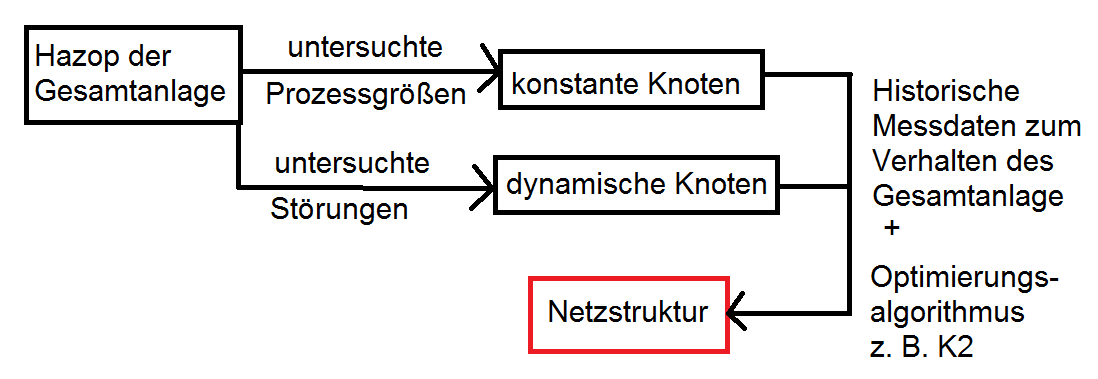
\includegraphics[width=0.5\textwidth]{bilder/Hu_2015_Netzentstehung.png}
\caption{Erstellung eines Dynamischen Bayesschen Netzes}
\label{fig:Hu_2015_netzentstehung}
\end{center}
\end{figure}

\subsubsection{\cite{Cai_2015}} Resiliente Systeme, Verwendung eines \ac{hfpm} als Erweiterung der \ac{irml}. Ziel des Modells ist die Beschreibung des dynamischen Verhaltens und die dynamische Fortpflanzung von Fehlern. Des neue Modell hat zwei Teile: statische Analyse der Struktur und dynamische Analyse f\"ur Fehlerfortpflanzung. Untersucht werden Fehler durch Abweichungen von Stoffparametern und Ger\"ateausf\"alle. Der Fokus liegt auf der Analyse der Resilienz (F\"ahigkeit des Systems trotz Fehler in definierten Zustand zu gelangen). \linebreak

Wird eine \ac{hazop} um ein Strukturmodell erg\"anzt, so kann eine Fehleranalyse systematisch durchgef\"uhrt werden ( Boonthum et al., 2014 ). Eine \ac{hazop} erfasst aber nur die Abh\"angigkeit von Prozessgr\"o\ss{}en und nicht die der Komponenten eines Systems, eine makroskopische Betrachtung von Fehlerfortpflanzungen ist daher nicht m\"oglich. Die folgenden Methoden zur makroskopischen Betrachtung werden genannt: 
\begin{itemize}
\item Utne et al. (2011): cascade diagram
\item Johansson and Hassel (2010): agent based approach $\mapsto$ ben\"otigt detaillierte Prozesskenngr\"o\ss{}en und Messwerte, quantitativ
\item  Kj{\o}lle et al. (2012) across-sector approach $\mapsto$ ben\"otigt vielseitiges Wissen und umfangreiche Daten \"uber den Prozess, diese sind oft nicht vorhanden
\item Haimes and Jiang (2011) Framework basierend auf Leontief’s input-output model $\mapsto$ ungeeignet f\"ur die Analyse von Verkn\"upfungen auf Komponentenebene
\item SDG \textcolor{green}{insbesondere in Verbindung mit \ac{hazop}}
\item Functional Resonance Analysis Method (FRAM) $\mapsto$ emphasizes the functional relationship between components and provides a way to describe the fault evolution
\item fault semantic network (FSN) using genetic programming (GP) and neural networks (NN) $\mapsto$ braucht viele Daten und Prozesswissen
\item Petrinetze
\item hierarchical Bayesian model (HBM)
\item Markov network combined with Bayesian theory
\end{itemize}
Vorteile \ac{hfpm}: \begin{enumerate}
\item Fehleranalyse auf Systemebene (statt Komponentenebene)
\item durch Simulation k\"onnen im vorweg geeignete Sicherheitsma\ss{}nahmen ermittelt werden, um gew\"unschte Sicherheitslevel zu erreichen
\end{enumerate}
Systemaufbau: \begin{itemize}
\item basierend auf \ac{irml}
\item ein System wird in Subsysteme gegliedert, die Struktur durch ein hierarchisches Framework dargestellt, die Gliederung in mehrere Ebenen von Subsystemen stellt die Prozessstruktur und Fehlerszenarien dar
\item statische Analyse: zeigt den Grad der Abh\"angigkeit von Subsystemen auf, das System wird auf die Teile mit den st\"arksten Wechselwirkungen reduziert und diese Teilsysteme werden im Detail weiter untersucht
\item dynamische Analyse: Anwendung von Testf\"allen; durch Wenn--dann Analyse werden die Fortpflanzung eines bekannten Fehlers und die Operationen des Systems, welche notwendig sind, um in einen stabilen Zustand zur\"uck zu kehren, im Modell so eingestellt, dass das Verhalten dem Testfall entspricht, mit Hilfe geeigneter Parameter, welche vor allem das zeitliche Verhalten widerspiegeln, wird das Verhalten gekennzeichnet und darauf aufbauen ein Zustandsgraph ermittelt
\end{itemize}

\textcolor{green}{Fazit: statische Analyse ist hilfreich, bietet aber keinen besonderen Mehrwert, dynamische Analyse erforderte historische Messdaten, Aufteilung auf Module ist fragw\"urdig, Analyse der anf\"alligsten Subsysteme ist hilfreich, Fokus liegt auf Resilienz und Berechnungen zum Sicherheitslevel insbesondere w\"ahrend ein Fehler sich im System verbreitet und das System darauf reagiert, f\"ur meine Arbeit eher nicht zu gebrauchen}
\textcolor{red}{die verwiesenen Methoden zur makroskopischen Betrachtung k\"onnten hilfreich sein.}

\subsubsection{\cite{Mallick_2013}} Entwicklung einer echtzeitf\"ahigen Methode zum Erkennen des Vorliegen eines Fehlers und Identifikation der Grundursache. Verwendung von \ac{pca} in Kombination mit \ac{bbn}. Aus Daten zum Normalbetrieb wird das \ac{pca} aufgebaut. Im laufenden Betrieb kann dann damit das Vorliegen eines Fehlers erkannt werden. Mit Hilfe historischer Daten zur Prozessdynamik oder durch Formulierung von Differentialgleichungen oder durch Expertenwissen wird das \ac{bbn} aufgestellt. Auf Basis des \ac{bbn} kann bei vorliegen eines Fehlers dessen Ursache ermittelt werden. Das initiale \ac{bbn} wird mit fortschreitender Betriebszeit durch Informationen aus der \ac{pca} verbessert um die Ursachenanalyse genauer zu machen.  

\textcolor{green}{Sch\"one Methode, welche statische Verfahren (\ac{pca}) mit Prozesswissen (\ac{bbn}) vereint, die ben\"otigten Daten zum Gesamtprozess, welche f\"ur \ac{pca} notwendig sind, liegen bei modularen Anlagen aber nicht vor $\mapsto$ bringt nichts}

\subsection{Rezensionen}
\begin{itemize}
\item Einf\"uhrung in \cite{Zhang_2017}: \textcolor{green}{\"Ubersicht datenbasierte Methoden}
\item Einf\"uhrung in \cite{Yang_2010}: \textcolor{green}{Entwicklung von Methoden zu \ac{sdg}}
\item Einf\"uhring in \cite{Mallick_2013}: \textcolor{green}{Verweise auf mehrere Methoden/Anwendungen von \ac{sdg}}
\item Einf\"uhrung in \cite{Cai_2015} \textcolor{red}{Methoden zur makroskopischen Fehlerfortpflanzung $\mapsto$ genau das will ich eigentlich }
\item Einf\"uhrung in \cite{Wang_2016}: Datenbasierte Fehlerfortpflanzung
\item \cite{Thornhill_2006}: Datenbasierte Fehlerfortpflanzung
\item \cite{Yin_2014}: Datenbasierte Fehlerfortpflanzung
\item \cite{Varga_2013}: Datenbasierte Fehlerfortpflanzung
\item \cite{Hwang_2010}: Modellbasierte und stochastische Methoden der Fehlerfortpflanzung; Reglerneueinstellung nach Fehlererkennung
\item \cite{Ng_2010}
\item \cite{Zhang2008} \textcolor{green}{Umfassende \"Ubersicht zum Thema Fehlerfortpflanzung und Fehleridentifikation}
\item \cite{Yang2012}
\item \cite{Duan2014}: \textcolor{green}{Ursachenanalyse von anlagenweiten, schwingenden Fehlern}
\item Einf\"uhrung in \cite{Li_2016}: \textcolor{green}{\"Ubersicht zu datenbasierten Methoden}
\item \cite{Venkatasubramanian_2003}: \textcolor{green}{quantitative modellbasierte Methoden}
\item \cite{Venkatasubramanian_2003a}: \textcolor{green}{qualitative modellbasierte Methoden}
\item \cite{Venkatasubramanian_2003b}: \textcolor{green}{datenbasierte Methoden}

\end{itemize}


\subsection{unsortiert}
\paragraph*{\cite{Bartolozzi_2000}} Qualitative models of equipment units and their use in automatic {HAZOP} analysis

%\subsubsection{\cite{Kavcic_2001}}
%Verfahren zur Fehlerbetrachtung werden in off-line und on-line Modelle unterschieden. Off-line sind bspw. \ac{hazop}, \ac{fta}, \ac{fmea}. On-line Verfahren basieren auf statistischen Methoden oder Mustererkennung.  

%\section{Modularisierung}

%\paragraph*{\cite{Bramsiepe_2012}} Sichtweisen auf die Modularisierung chem. Produktionsanlagen. Anforderungen an Module. Grundlegende Gedanken und notwendige Schritte zur Verwendung von Modulen. \hfill \newline
%Verk\"urzte Lebenszyklen chemischer Produkte und st\"arker schwankende Absatzm\"arkte erfordern k\"urzere Entwicklungszeiten neuer Produkte. Modularisierte Anlagenteile wurden als m\"ogliches Mittel identifiziert, um bereits gewonnenes Wissen wiederverwenden zu k\"onnen und so Entwicklungszyklen zu beschleunigen. Aus wirtschaftlicher Sicht konnte die Sinnhaftigkeit kleinskaliger Anlagen bereits gezeigt werden (Quellen sie diese Arbeit). Diese erlauben hohe Flexibilit\"at und eine schnelle Anpassung der Produktionskapazit\"at an Marktver\"anderungen. Mit Hilfe kleinskaliger Anlagen k\"onnen insbesondere Zwischenprodukte einzeln und \"ortlich verteilt hergestellt werden. Die Weiterverarbeitung zu einem Endprodukt erfordert dann nur noch den Transport dieser Zwischenprodukte und nicht mehr den Transport aller Ausgangsstoffe. Dadurch sinkt das zur Endproduktgewinnung notwendige Transportvolumen und damit die Kosten. Ein weiterer Vorteil der Modularisierung ist die M\"oglichkeit einen Gro\ss{}teil der Anlagenmontage an einem beliebigen Ort unter optimalen Bedingungen vornehmen zu k\"onnen. Am Aufstellungsort der Anlage m\"ussen die Module dann nur noch verbunden werden. Dies ist insbesondere bei klimatisch anspruchsvollen Anlagenstandorten sehr hilfreich. Ein Modul muss derart definiert werden, dass es einen hohen Grad an Wiederverwendbarkeit besitzt und l\"osgel\"ost von einer Gesamtanlage getestet werden kann. Module sollten nach ihrem Detaillierungsgrad unterschieden werden. Die Aufteilung in Planungsmodule und Variantenmodule wird als sinnvoll erachtet. Variantenmodule werden in 2D und 3D Varianten unterteilt. Ein 2D Variantenmodul soll Informationen enthalten, welche am Ende des Basic Engineering vorhanden sind. Dies umfasst alle Informationen, welche zum Entwurf eines R\& I Flie\ss{}bildes f\"ur ein Modul notwendig sind. Ein 3D Variantemodul ist um Auslegungsgr\"o\ss{}en derart erweitert, dass die Modulfertigung m\"oglich ist. Weiterhin sind der Planungs- und Entwicklungsprozess geeignet dokumentiert. Die konkrete Auslegung der 3D Variantenmodule kann direkt durch einen Equipmentlieferanten durchgef\"uhrt werden, wenn dieser detaillierte Modulanforderungen und Raumforderungen erh\"alt. Insbesondere eine genau Definition der Schnittstellen ist hierbei notwendig.  
%Ein Planungsmodul bietet Ans\"atze zu Auswahl, Funktionsumfang, Auslegung und Dimensionierung von Variantenmodulen. Planungsmodule stellen also in erster Linie einen Wissensspeicher dar und dienen der Darstellung der Vielfalt von Variantenmodulen. Wird durch einen Wissens-/ Erfahrungsgewinn ein bestehendes Variantenmodul weiterentwickelt, so m\"ussen die Planungsmodule erweitert und angepasst werden.
%Im Planungsprozess hat der Detaillierungsgrad der verwendeten Variantenmodule ma\ss{}geblichen Einfluss. 2D Module erleichtern die Erzeugung von Flie\ss{}bildern einer Gesamtanlage. Insbesondere erm\"oglichen sie den einfachen Vergleich verschiedener Anlagenstrukturen. Es wird auf Literatur verwiesen, welche die zur Erlangung von 2D und 3D Modulen notwendigen Arbeitsschritte darlegen. Mit Hilfe von Simulationen k\"onnen in Kombination mit Planungsmodulen geeignete 3D Module f\"ur einen Prozess ausgew\"ahlt werden. Da diese nur in definierten Gr\"o\ss{}en zur Verf\"ugung stehen wird der Prozess aber wahrscheinlich nicht optimal umgesetzt. Dies muss bei der Planung beachtet werden, z. B. indem der Verfahrensprozess an vorhandene Modulgr\"o\ss{}en angepasst wird. Auf ein solches Vorgehen wird verwiesen (\cite{Seifert_2012}). Bei der Entwicklung von Regelungs- und Sicherheitskonzepten muss betrachtet werden, welche Aufgaben ein einzelnes Modul losgel\"ost vom Gesamtsystem erf\"ullen kann und welche Aufgaben nur im Zusammenspiel mehrerer Module gel\"ost werden k\"onnen. Die implementierten F\"ahigkeiten des Module bestimmen also ma\ss{}geblich den Entwicklungsaufwand neuer Sicherheitsfunktionen einer Gesamtanlage. 
%Die einzelnen Schritte der Projektplanung \"uerlappen sich bei der Verwendung von Modulen zwangsl\"aufig. Um eine effiziente und effektive Projektplanung sicherzustellen ist daher die Entwicklung eines geeigneten Datenformates notwendig. Nur so kann eine st\"andige Weitergabe und Verf\"ugbarkeit notwendiger Information gew\"ahrleistet werden.  
%Notwendige Forschungsarbeiten, um Module verwenden zu k\"onnen: \begin{itemize}
%\item Systematischer Entwurf von 2D, 3D Variantemodulen und Planungsmodulen(Systematik des Modulentwurfs definieren)
%\item Berechnungsmodelle zum Scale-Up von Modulen
%\item Simulationsmodelle von Modulen, um deren Variantenauswahl und konkrete Auslegung durchf\"uhren zu k\"onnen
%\item (Weiter-) Entwicklung von Ans\"atzen, wie Module konkret in den Planungsprozess integriert werden k\"onnen
%\item Entwicklung eines Datenmodell um Datenaustausch und Datenanreichung zu erm\"oglichen
%\end{itemize}
%\hfill \newline
%\textcolor{green}{Inhaltlich fertig.} \textcolor{red}{Arbeiten, welche diesen Artikel zitieren, sind wahrscheinlich hilfreich}.

%\paragraph*{\cite{Kampczyk_2003}}
%Vorstellung eines CAE-Tools zur Anlagenplanung, insbesondere zur Wahl der Positionierung von Anlagenkomponenten, Entwicklung der Vorrohrung und dem Stahlbau. Durch Vorgabe von Nutzerw\"unschen wird auf Basis einer Wissensdatenbank die optimale Positionierung und Leitungsf\"uhrung berechnet, indem alle Varianten (oder eine definierbare Anzahl an Iterationen) an m\"oglichen Kombinationen automatisch durch einen Optimierer berechnet und bewertet wird. Durch Definition von Modulen wird die Anzahl m\"oglicher Varianten reduziert und der Rechenaufwand reduziert. Au\ss{}erdem k\"onnen best-practice L\"osung direkt vorgegeben werden. \hfill \newline
%Modul $=$ Ausr\"ustungen, welche Teil des gleichen Prozessschrittes sind. \textcolor{red}{Diese Arbeit hilft die verschiedenen Verst\"andnisse vom Modulbegriff darzulegen}.

%\paragraph*{\cite{Hady_2012}}
%Das vorgestellte Konzept umfasst die Definition und Identifizierung von Modulen, deren dreidimensionales Design, die Ablage und Know-how-Sicherung zwecks der Wiederverwendung des Engineering und der Ausrüstungen sowie die Planung und Kostenschätzung mit wiederverwendbaren Modulen.\textcolor{red}{Arbeiten, welche diesen Artikel zitieren, sind wahrscheinlich hilfreich}.

%\paragraph*{\cite{Urbas_2012}} \textcolor{red}{\"Ubersichtsbeitrag Modularisierung, offene Forschungsfragen}

%\paragraph*{\cite{Lier_2016}} Relevanz modularisierter Anlagen
%
%\paragraph*{\cite{Obst_2013}} Relevanz modularisierter Anlagen
%
%\paragraph*{\cite{Ohle_2014}} Konkretes Beispiel einer Modularen Anlage


 
% \paragraph*{\cite{Uzuner_2012}, \cite{Uzuner_2013}} Ans\"atze im Paper, Details in der Dissertation \hfill \newline
%Die Entwicklung des R{\&}I-Flie{\ss}bild ist ein wichtiger Schritt eines Anlagenprojektes. In der Arbeit wird gezeigt, wie dieser Prozess durch Unterteilung einer Gesamtanlage in wiederverwendbare Funktionsgruppen (=Module bzw. EQM) und die Verwendung einer wissensbasierten Software geeignet beschleunigt werden kann. Module sollen derart definiert werden, dass sie prozesstechnisch sinnvoll sind und einen m\"oglichst hohen Grad an Wiederverwendbarkeit aufweisen. Ein solches Modul wird als Equipment-Modul (EQM) bezeichnet; gemeint sind damit Standard-Prozesseinheiten wie Pumpen, Verdichter, W\"arme\"ubertrager, Beh\"alter, Reaktoren, Kolonnen. Ein EQM erf\"ullt dann eine prozesstechnische Funktion und umfasst einen Apparat/Eine Maschine und weiterhin die notwendigen Elemente der Sicherheitstechnik, Regelungstechnik, Nahverrohrung und Instrumentierung. F\"ur solche EQM wurden R{\&}I-Flie{\ss}bilder entworfen. Ein EQM kann dabei in Subsysteme zerlegt werden, welche derart definiert werden, dass sie anschlussfertige Elemente f\"ur EQM bilden (z. B. Teilmodul, Baugruppe, Unterbaugruppe). Diese Verschachtelung erfordert eine Erweiterung der \textcolor{red}{NE33 - Datei besorgen}. Der Zusammenbau eines EQM zur Erf\"ullung einer bestimmten Funktion kann durch Kombination verschiedener Subsystemen geschehen (verschiedene Kombinationen bilden verschiedene EQM zur Erf\"ullung der gleichen Aufgabe). Dadurch k\"onnen neue oder abge\"anderte Prozesse flexibel realisiert und Variationen eines EQM bez\"uglich der Kosten verglichen werden. Bereits entworfene EQM bilden die Basis der wissensbasierten SW. Neue EQM und deren Subsysteme erweitern die SW. Neue Anlagen werden dann aus diesem Datenhaushalt - den bereits geplanten Modulen - entworfen, oder die Datenbasis wird zuerst erweitert. Bereits geleistete Entwicklungsarbeit kann so wiederverwendet werden. Durch die Verwendung von Standardbausteinen sinkt die Entwicklungsdauer, wird die Qualit\"at der Planungsarbeit erh\"oht, erlangtes Wissen nachvollziehbar gespeichert und die Dokumentation von Designentscheidungen erleichtert. Die Struktur der SW und die Handhabung/ der Nutzen der SW im Workflow werden erl\"autert. Der Planungsgrad ist auf 2-D Level. Die r\"aumliche Anordnung von Komponenten eines EQM wird nicht betrachtet/ modelliert. \textcolor{green}{fertig}

%\paragraph*{\cite{Lang_2012}} Die aus Standard-Modulen aufgebaute Anlage hat sich bisher noch nicht im gro\ss{}en Ziel durchgesetzt. Im Bereich der Kleinanlagen ist die Entwicklung von Containermodulen jedoch weit voran geschritten. Es existiert bereits wenigstens ein kommerzielles Produkt - der \textit{Evotrainer}. \textcolor{green}{fertig}

%\paragraph*{\cite{Rottke_2012}} Am Beispiel einer Anlage zur Hochleistungsfl\"ussigkeitschromatographie (welche in der Literatur detailliert beschrieben ist) wird gezeigt, wie der Ansatz der modularisierten Anlage praktisch genutzt werden kann. Der Prozess wird in Module zerlegt, welche in verschiedenen Skalierungsvarianten entworfen werden. Die zus\"atzlichen Kosten, wenn ein Modul in Zwischengr\"o\ss{}e ben\"otigt wird, wird dargelegt. Es wird ein Paket an Werkzeugen vorgestellt, mit Hilfe derer die ben\"otigte Dimensionierung von Modulen f\"ur einen Prozess durch Simulation berechnet wird und eine kostenbasierte Empfehlung abgegeben, welche Modulvariante aus einem Katalog definierten Gr\"o\ss{}en gew\"ahlt werden sollte. \hfill \newline
%Ein Ansatz der deutschen Anlagenbauer und -betreiber ist die Entwicklung von High--Tech--Produkten um im globalen Wettbewerb erfolgreich zu bleiben. Dazu ist unter anderem eine stark verk\"urzte Projektzeit bei der Entwicklung neuer Produkte notwendig. Die Verwendung von Modulen bei der Prozessentwicklung ist ein m\"oglicher Ansatz. Im ersten Schritt ist allerdings ein erh\"ohter Engineering Aufwand zur Definition und Erstellung/Beschreibung von Modulen notwendig. Dieser Mehraufwand ist gerechtfertigt, wenn ein entworfenes Modul mehrfach verwendet werden kann. Die erbrachte Engineering--Leistung kann damit wiederverwendet werden. Insbesondere die Dokumentation, wie ein Modul entstanden ist (die konkreten Designentscheidungen) ist daf\"ur notwendig.  \hfill \newline
%Das R{\&}I-Flie{\ss}bild wird so erstellt, dass einzelne Komponenten (die Module) frei ausgetauscht werden k\"onnen. Module m\"ussen also \"uber definierte Schnittstellen verf\"ugen und klar definierte Verfahrenstechnische Prozessschritte erf\"ullen. Weiterhin sollten Module einzeln testbar und skalierbar sein. Wurde eine Anlage so geplant, dass Module austauschbar sind, so kann ein erh\"ohter Bedarf an Produktionsmenge durch Skalierung der Module befriedigt werden. Module sollten daher in definierten Gr\"o\ss{}en entworfen werden. Je nach Anwendungsfall wird dann die am Besten passende Gr\"o\ss{}e ausgew\"ahlt. Der Prozess wird dadurch nicht mehr optimal erf\"ullt (das Modul wird immer etwas \"uberdimensioniert sein, je nach dem wie weit die n\"achte Modulgr\"o\\ss{}e von der eigentlich erforderlichen Gr\"o\ss{} weg ist), daf\"ur l\"auft die Planung aber deutlich schneller ab. Am Beispiel der Hochleistungsfl\"ussigkeitschromatographie wird gezeigt, wie ein Verfahren in Module zerlegt werden kann. Die Module werden f\"ur verschiedene Produktionsmengen entworfen (also Stufenweise). Die Auswirkung auf die Kosten einer Anlage mit nicht-optimalen Modulen bzgl. der Gr\"o\ss{} wird dargelegt. Nachteil einer modularen Bauweise ist, dass sonderw\"unsche von Kunden nur kompliziert erf\"ullt werden k\"onnen. Im Fall von Defekten ist ein Austausch von Ger\"aten daf\"ur wesentlich preiswerter, da eben keine Sonderanfertigungen gemacht werden. Ein Anlagenhersteller gelangt durch die wiederholte Verwendung eines Moduls au\ss{}erdem zu mehr Erfahren/ Detailwissen und kann damit Bedienbesonderheiten und Anwendungspotential eines Moduls besser ausssch\"opfen (und dieses Wissen an den Anlagenbetreiber weiter geben). Insbesondere Schulungen zum Betrieb der Anlage sind fr\"uzeitig im Entwicklungsprozess m\"oglich. Der Prozess wird daher sicherer (lernen aus Erfahrung einfacher, vor allem bzgl. Bedienung und Designfehlern). Zus\"atzlich werden Module vom Layout her bez\"uglich Kosten und Funktion optimiert. Man erkauft sich also durch eine \"Uberdimensionierung der Anlage bez\"uglich der notwendigen Gr\"o\ss{}e (da Gr\"o\ss{}e nicht optimiert wird) durch eine schnelle Planung und Module, welche ihre Funktion optimal erf\"ullen, ein optimales Layout haben und durch mehr Erfahrung besonders sicher sind. Liegt eine erforderliche Modulgr\"o\ss{}e zu weit weg von bereits designten Modulgr\"o\ss{}en, so wird das bekannte Modul sinnvollerweise neu skaliert oder der Kunde lebt mit nicht-optimalem Prozess. Bei Neu-Skalierung kann vorhandenes Wissen \"uber Layout des Moduls aber wieder verwendet werden -> ist also nicht sooo schlimm. 

%\paragraph*{\cite{Obst_2013b}} Automatisierung im Life Cycle modularer Anlagen
%
%\paragraph*{\cite{Urbas_2012a}} Automatisierung von Prozessmodulen

%\paragraph*{\cite{Fleischer_2016}} Planungsansatz f{\"u}r modulare Anlagen in der chemischen Industrie. Viele Literaturreferenze, sehr aktueller Text zur Problematik der Verwendung von modularen Anlagen in der Industrie

%\paragraph{\cite{Lier_2016a}} Transformable Production Concepts: Flexible, Mobile, Decentralized, Modular, Fast: Bereits verwendete Konzepte werden vorgestellt (F3, Evotrainer, Copiride), die Notwendigkeit modularer Anlagen wird dargelegt, Arbeiten zur Wirtschaftlichkeit werden ausgewertet mit dem Schluss, dass sich besonders bei kurzen Produktlebenszyklen der Einsatz modularer Anlagen lohnt.  

%\paragraph*{\cite{Hohmann_2017}} Modules in process industry - A life cycle definition

%\subsection{Moduldarstellung}

%\paragraph*{\cite{Wassilew_2017}}

%\paragraph*{\cite{Obst_2015}} Beschreibung von Prozessmodulen
%
%
%\paragraph*{\cite{Wassilew_2016}}
%Zur Darstellung von Modulen wird ein MTP erstellt. Dies entspricht dem in NAMUR vereinbarten Anforderungen? Der Informationsgehalt des MTP kann automatisiert in das Format von OPC UA transformiert werden. Wie das geht, steht in dieser Arbeit.


%\paragraph*{\cite{Obst_2015a}} Semantic description of process modules

%\section{Mini- und Milliplanttechnik}
%
%\paragraph*{\cite{Grundemann_2012}} Relevanz von Mikroreaktoren und deren Beziehung zur 50 Prozent These anhand zweier Beispiele.
%
%\paragraph*{\cite{Brodhagen_2012}} Kostenvorteil durch Modularisierung von Anlagen, insbesondere bei Verwendung von Mikroreaktoren anhand einer Fallstudie. \hfill \newline
%Es gibt einen Trend zu kundenspezifischen Produkten, welche die Massenprodukte zunehmend ersetzen. Der Umfang umfasst nur bis zu wenigen tausend Tonnen pro Jahr. Die Lebenszyklen solcher Produkte betragen au\ss{}erdem nur wenige Jahre. Eine kurze Entwicklungszeit ist daher von hoher Wichtigkeit, um wettbewersbf\"ahig zu bleiben. Weiterhin ist die Flexibilit\"at einer Anlage ausschlaggebend. 
%Batchprozesse haben folgenden Nachteile: \begin{itemize}
%\item Scale-Up ist schwierig, da insbesondere die W\"armeabfuhr bei gro\ss{}en Reaktoren wesentlich schlechter als im Laborma\ss{}stab ist. Dies f\"uhrt bei stark exothermen Reaktionen zu Sicherheitsproblemen und vergr\"o\ss{}ertem Planungsaufwand
%\item Batchanlagen sind nicht sehr flexibel. Durch feste Chargengr\"o\ss{}en m\"ussen bei geringen Absatzmengen Zielstoffe und Ausgangsstoffe in gro\ss{}en Mengen zwischengelagert werden, um verschiedene Produkte herstellen zu k\"onnen und die Anlage voll auszulasten.
%\end{itemize}
%Milli-Reaktoren bieten eine Alternative. Sie sind gekennzeichnet durch einen kontinuierlichen Betrieb, Str\"omungskan\"ale mit Durchmessern im Millimeterbereich und sehr hohen W\"armeaustauschfl\"achen pro Volumeneinheit (ca. Faktor 100 zu klassischen Anlagen), wodurch die W\"arme bei stark exothermen Reaktionen gut abgef\"uhrt werden kann, was eine inh\"arente Sicherheit zur Folge hat. 
%Um ein einfaches Scale-Up von neuen Prozessen zu erm\"oglichen m\"ussen Anlagen im Produktionsma\ss{}stab m\"oglichst die gleichen Eigenschaften wie solche in Laborgr\"o\ss{}e aufweisen. Entwickelte Prozesse m\"ussen dann nicht aufwendig angepasst werden und der Entwicklungsprozess wird stark beschleunigt. Milli-Reaktoren bieten diese Eigenschaft. Au\ss{}erdem k\"onnen mit ihnen hohe Raum-Zeit Ausbeuten erreicht werden. Milli-Reaktoren k\"onnen flexibel eingesetzt werden und sind besonders f\"ur einen modularen Aufbau geeignet. Durch Parallelisierung mehrerer Milli-Reaktoren k\"onnen Produktionskapazit\"aten flexibel angepasst werden und damit auf Marktver\"anderungen effizient reagiert werden. Mit Hilfe einer Kapitalwertanalyse wird an einem Fallbeispiel das Potential von Milli-Reaktoren nachgewiesen. Es wird ein linear wachsender Mark f\"ur ein neu entwickeltes Produkt angenommen.  Es wird gezeigt, dass eine Aufteilung von Produktionskapazit\"aten durch die Verwendung von Modulen insbesondere bei kurzen Produktlebenszeiten (bis 10 Jahre) sinnvoll ist. Die h\"oheren Betriebskosten mehrere Module werden dabei durch optimierte Produktionsmengen ausgeglichen. Der Bau von Gro\ss{}anlagen rentiert sich erst bei l\"angeren Produktlebenszyklen oder bei extrem schnell wachsender Produktnachfrage. Weiterhin wird gezeigt, dass eine Zeiteinsparung bei der Produktentwicklung h\"ohere Entwicklungs- und Investitionskosten durch die Verwendung von Milli-Reaktoren rechtfertigt und zu einem wirtschaftlich besseren Ergebnis als die Verwendung von Batch-Prozessen f\"uhrt. 
% \textcolor{green}{fertig}


%\paragraph*{\cite{Kockmann_2012}} Hochskalieren von Anlagen mit Hilfe modularer Konzepte und Mikroreaktoren. \hfill \newline
%Basierend auf Kennzahlen für die Reaktionskinetik und - enthalpie wird eine \textcolor{red}{Korrelation} abgeleitet und mit der konvektiven Wärmeübertragung als ein Kriterium des \textcolor{red}{sicheren Reaktorbetriebs} gekoppelt.

%\paragraph*{\cite{Sell_2013}}
%\textit{Alles nur zitiert!} \hfill \newline
%Die Ergebnisse bisheriger vergleichender Kostenanalysen zwischen diskontinuierlich betriebenen chemischen Verfahren und deren mikroverfahrenstechnischem Pendant haben gezeigt, dass letztere nicht pauschal als kosteneffizientere Alternative gesehen werden können. Es bedarf, wie auch bei Batch-Prozessen, einer umfassenden Prozessoptimierung und Effizienzmaximierung. Dann können mikroverfahrenstechnische Prozesse jedoch trotz teilweise höherer Investitionskosten aufgrund geringerer laufender Kosten und einem schnelleren Zugang zum Markt die ökonomisch günstigere Alternative darstellen. \textcolor{red}{Relevanz von Mikroanlagen}

%\paragraph*{\cite{Hessel_2012}}Potenzialanalyse von Milli- und Mikroprozesstechniken
%
%\paragraph*{\cite{Behr_2012}} Vorteile der Miniplant-Technik im Hinblick auf eine effiziente Verfahrensentwicklung anhand von Beispielen homogen katalysierter Verfahren. Literaturverweise auf alle genannten Vorteile und Eigenschaften von Miniplants. \hfill \newline
%Experimentelle Untersuchungen in unterschiedlichen Ma\ss{}st\"aben nehmen den gr\"o\ss{}ten Teil der Zeit w\"ahrend der Prozessentwicklung ein. Zum Beginn der Prozessentwicklung wird meist mit Batchprozessen gearbeitet, um die Einfl\"usse von Z. B. Katalysatoren, Aktivatoren, Druck, Temperatur usw. untersuchen zu k\"onnen. Eine Vielzahl industrieller Prozesse wird jedoch kontinuierlich durchgef\"uhrt. Ein reines Scale-Up einer Batchanlage reicht daher nicht aus. Statt dessen muss im Laufe der Prozessentwicklung eine kontinuierliche Pilotanlage entworfen werden und der Prozess teilweise neu untersucht werden. Statt diesem Entwicklungsprozess kann eine hochflexible Miniplant im Laborma\ss{}stab mit Hilfe von standardisiertem Laborequipment in kurzer Zeit und mit geringen Kosten entworfen werden. Diese wird bereits kontinuierlich betrieben und an ihr kann der Prozess entwickelt und in Echtzeit untersucht werden. Miniplants existieren mit Scale-Up Faktoren von bis zu 10000 und mehr. Apparate Volumina liegen im Bereich weniger Liter, Durchsatzmengen bis zu $1 \frac{kg}{h}$. Die Prozessentwicklung mit Hilfe kontinuierlicher Reaktoren erlaubt insbesondere eine genaue Betrachtung der Einfl\"usse verschiedener Prozessparameter, da station\"are Arbeitspunkte und Schwankungen um diese gezielt untersucht werden k\"onnen. Au\ss{}erdem kann die wirtschaftlich h\"ochst relevante R\"uckgewinnung von Katalysatoren und die R\"uckf\"uhrung von Stoffen - z. B. die R\"uckf\"uhrung von Nebenprodukten zur Steigerung der Ausbeute gew\"unschter Stoffe - geeignet untersucht werden. Auf geeignete Literatur zu dieser Thematik wird in der Arbeit verwiesen. Weiterhin sind Miniplants zur Personalschulung und der \"Uberpr\"ufung der Einhaltung von Industriestandards nutzbar. Die Korrektur von Fehlern im Prozess ist im Rahmen einer Miniplant wesentlich preiswerter als bei Verwendung einer Pilotanlage. \cite{Krekel_1985} Mit Hilfe komplexer Simulationen ist ein Scale-Up der Miniplant auf Produktionsniveau bei vielen Prozessen direkt m\"oglich. Nur noch kritische Prozesseinheiten m\"ussen im Pilotma\ss{}stab gesondert untersucht werden. Die Umgehung einer kompletten Pilotanlage spart mehrere Jahre Entwicklungszeit. Au\ss{}erdem werden hohe Kosten bei Planung und Betrieb einer Pilotanlage eingespart. Die erfolgreiche Untersuchung und Entwicklung von Prozessen mit Hilfe einer Miniplant wird an vier Beispielen ausgef\"uhrt. Der Fokus liegt dabei auf der R\"uckgewinnung eingesetzter Katalysatoren. 
%\hfill \newline
% \textcolor{green}{fertig}
% 
% \paragraph*{\cite{Helling_2012}} Die Verwendung von Mikroprozessen ist eine relativ neue und weiterhin wachsende Technologie. Ihren Durchbruch hatte diese Technologie in den fr\"uhen und mittleren neunziger Jahren. Die Forschung konzentriert sich derzeit auf die Umwandlung von Batch-Prozessen in Kontinuierliche durch Verwendung modularer Mikro- und Minireaktoren, mit Hilfe derer die Entwicklungszeit neuer Anlagen drastisch gesenkt werden soll. Vorteile sind ein erh\"ohter Stoffaustausch und eine verbesserte W\"arme\"ubertragung. Durch die geringen Stoffvolumina in Mini- bzw. Mikroreaktoren steigt automatisch die Sicherheit besonders von exothermen Reaktionen. Dadurch werden Verfahren m\"oglich, die in konventionellen Reaktoren nur durch hohen Aufwand oder garnicht durchf\"uhrbar w\"aren. Mini- und Mikroanlagen mit gleicher Funktion k\"onnen prinzipiell aus verschiedenen Werkstoffen hergestellt werden. Typisch sind Glas, Keramiken und Edelstahl. Einige Typen sind W\"armetauscher (welche die ersten Mikroanlagen waren), Fallfilmreaktoren, m\"aanderf\"ormige Reaktoren und Photoreaktoren. \hfill \newline
%Bestehende Probleme sind das Design und die konkrete innere Geometrie von Mini- Mikroanlagen. Derzeit werden diese durch Versuch/ Fehler Verfahren in Kombination mit Erfahrungen aus bereits entwickelten Anlagen ermittelt. Eine exakte Reproduzierbarkeit der inneren Strukturen ist schwierig. Module vom gleichen Typ sind daher nicht unbedingt identisch im Verhalten. Soll durch die Verwendung mehrerer Module ein Hochskalieren von Stoffmengen umgesetzt werden, so ist dies daher kompliziert und oft nur bis zu gewissen Grenzen realisierbar. \hfill \newline
%Zum Zeitpunkt dieser Arbeit war insbesondere die Stofftrennung mit Hilfe von Mikroanlagen ein noch nicht komplett gel\"ostes Problem und daher Gegenstand aktueller Forschung. Die aktuelle Arbeit \cite{Yang_2017} gibt eine umfangreiche \"Ubersicht \"uber Entwicklungen zum Trennen von Stoffen durch Destillation mit Hilfe von Mikroanlagen. 
%
%\paragraph*{\cite{Kockmann_2012a}} Sicherheitsaspekte bei der Prozessentwicklung und Kleinmengenproduktion mit Mikroreaktoren



%\paragraph*{\cite{Kockmann_2014}} Micro Process Engineering: Fundamentals, Devices, Fabrication, and Applications

%\paragraph*{\cite{Sundberg_2014}} Micro-scale Distillation and Microplants in Process Development

%\paragraph*{\cite{Hugo_2009}}
%\textit{Alles nur zitiert!} \hfill \newline
%Reaktions- und sicherheitstechnische Aspekte der Umwandlung eines diskontinuierlichen
%chemischen Prozesses in ein kontinuierliches Verfahren unter Verwendung von Mikroreaktoren werden untersucht. Betrachtet man Mikroreaktoren als Module, so k\"onnte diese Arbeit interessant werden $\mapsto$ \textcolor{red}{das sollte ich daher fragen}. 

%\section{Weitere}

%\paragraph*{\cite{Seifert_2012}} Small scale, modular and continuous: A new approach in plant design. Wird bisher nur zitiert. 

%\paragraph*{\cite{Meier_2012}} Aus einer Reduktion der Planungszeit (welche Ziel der Verwendung von Modulen ist) kann nicht, wie man intuitiv meinen k\"onnte, allgemein auf eine Reduktion des Projektrisikos geschlossen werden. \textcolor{green}{fertig}.

%\paragraph*{\cite{Yang_2017}} wird im Text direkt zitiert, keine weitere Analyse notwendig.

%\paragraph*{\cite{Krekel_1985}} \textcolor{green}{wird nur zitiert}
%
%\paragraph*{\cite{Perkins_1992}} \textcolor{red}{hierin eine Quelle ab S. 215 bzw. 199}
%
%\paragraph*{\cite{Oppelt_2015}}
%Notwendigkeit von Simulation w\"ahrend dem Lebenszyklus einer Anlage

%\paragraph*{\cite{Strauch_2008}} Modulare Kostensch{\"a}tzung in der chemischen Industrie - Konzept eines integrierten Systems zur Absch{\"a}tzung und Bewertung des Kapitalbedarfes f{\"u}r die Errichtung einer chemischen Anlage

%\section{unsortiert}